\documentclass{beamer}
\usepackage[utf8]{inputenc}
\usepackage[T1]{fontenc}
\usepackage[ngerman]{datetime}
\renewcommand{\dateseparator}{..} % use dots instead of slashes to seperate dates
\usetheme{thk}
% custom colors:
% thk-red
% thk-orange
% thk-violet


\title{\LaTeX -Beamer Theme TH Köln}
\subtitle[Beispielpräsi]{Eine Beispielpräsentation}
\institute[TH Köln]{Technische Hochschule Köln}
% if a short version is given, this will be preferred in the footer. To use the long version, don't give a short version
\supervisor{Prof. Stefan Herzig} %leave empty if not applicable
% you can also use this tag for different purposes
\date[\ddmmyyyydate\today]{\today} %short date in brackets, long date in bracelets
\author[de Koster]{Markus de Koster}
\pagefooterlocalization{Seite } % can be anything, e.g. "Slide" "Page" "Seite"

\begin{document}

\begin{frame}
    \vspace{2em} %some distance to the top
    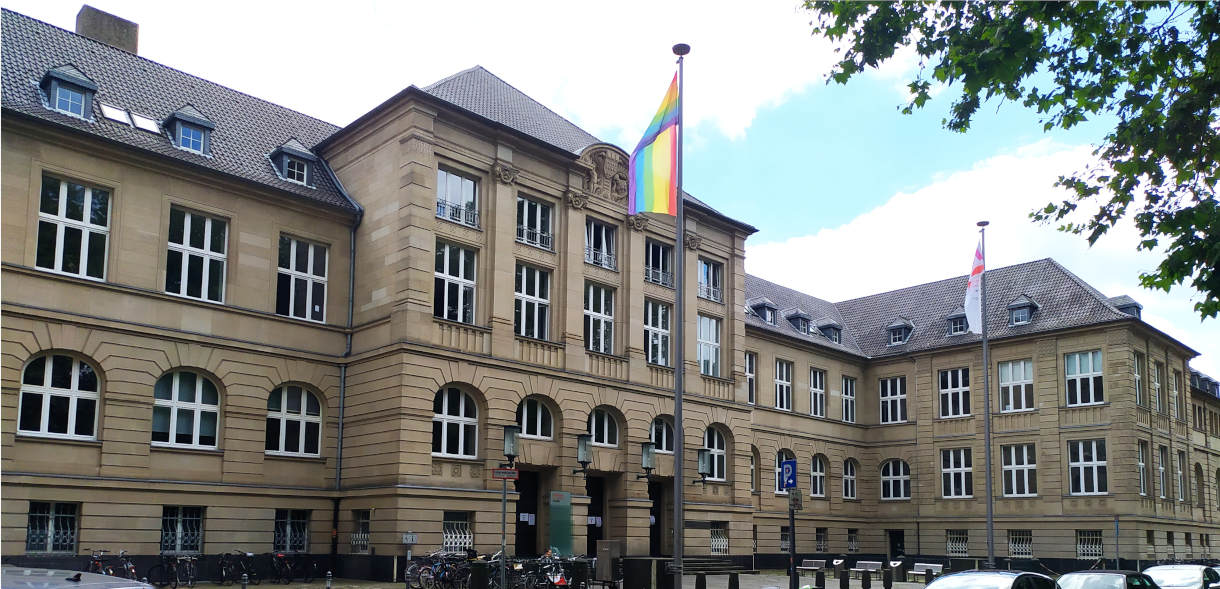
\includegraphics[width=\textwidth]{figures/thk.jpg}
    \titlepage
\end{frame}

\begin{frame}
    \frametitle{Inhalt}
    \tableofcontents
\end{frame}

\section{Wie sehen Aufzählungen aus?}\label{sec:enumerations}
\begin{frame} 
    \frametitle{Wie sehen Aufzählungen aus?} 
    \framesubtitle{Ein Beispiel für Aufzählungen} 
    \begin{theorem}
        Hier steht ein theorem oder Beispiel in default Farbe
    \end{theorem}

    % change the color of theorems from now on
    \AtBeginEnvironment{theorem}{%
        \setbeamercolor{block title}{use=example text,fg=white,bg=thk-orange}
        \setbeamercolor{block body}{parent=normal text,use=block title example,bg=block title example.bg!10!bg}
    }
    \begin{theorem}
        Hier steht ein zweites theorem in anderer Farbe
    \end{theorem}
    \begin{enumerate} 
        \item Hier steht ein item 
        \begin{enumerate} 
            \item Hier steht ein subitem
            \begin{enumerate} 
                \item Hier steht ein subsubitem
            \end{enumerate}
        \end{enumerate}
        \item Hier steht noch ein etwas längeres item, um den Zeilenumbruch zu zeigen. 
        Dieser wird automatisch gesetzt, sobald die Zeile zu lang wird.
    \end{enumerate}
\end{frame}

\subsection{Wie sehen Bulletpoints aus?}\label{sec:itemize}
\begin{frame}{Wie sehen Aufzählungen aus?}
\begin{itemize}
\item one
\begin{itemize}
    \item two
    \begin{itemize}
        \item three
    \end{itemize}    
\end{itemize}    
\item four
\end{itemize}
\end{frame}

\section{Grafiken}\label{sec:graphics}
\begin{frame}{Grafiken}
    \begin{figure}\label{thk-linien}
        
\includegraphics[width=\textwidth]{figures/thk-lines.png}
        \caption[TH Köln lines]{TH Köln lines. Adaptiert von \cite{source}}
    \end{figure}
\end{frame}

\end{document}